
\documentclass[11pt,a4paper]{article}

\usepackage[T1]{fontenc}
\usepackage[utf8]{inputenc}
\usepackage[dutch]{babel}
\usepackage{lmodern}
\usepackage{microtype}
\usepackage[a4paper,margin=2.0cm]{geometry}
\usepackage{amsmath,amssymb,bm}
\usepackage{booktabs,array,tabularx}
\usepackage{enumitem}
\usepackage{xcolor}
\usepackage{tikz}
\usetikzlibrary{arrows.meta,decorations.pathmorphing,positioning,calc,patterns,shapes.geometric,decorations.markings}

\definecolor{notegray}{RGB}{245,245,245}
\definecolor{uncertain}{RGB}{145,70,0}
\definecolor{inkblue}{RGB}{28,78,150}
\definecolor{inkred}{RGB}{190,45,45}
\definecolor{inkgreen}{RGB}{35,135,75}
\definecolor{inkpurple}{RGB}{115,60,145}

\newcommand{\uncertain}[1]{\textcolor{uncertain}{\textit{[onzeker: #1]}}}
\newcommand{\literalnote}[1]{%
  \begin{center}
  \fcolorbox{black!35}{notegray}{%
    \begin{minipage}{0.92\linewidth}
      #1
    \end{minipage}}
  \end{center}
}
\newcommand{\electron}[2]{\fill[inkblue!85] (#1,#2) circle (0.10);}
\newcommand{\proton}[2]{\fill[inkred!85] (#1,#2) circle (0.13);}

\title{\textbf{Kwantum Natuurkunde}\\
\large LaTeX-transcriptie van PDF-pagina's 21--25}
\author{}
\date{}

\begin{document}
\maketitle

\noindent
Deze transcriptie is gebaseerd op visuele inspectie van de oorspronkelijke
scans op hoge resolutie. Spelling en formulering zijn zoveel mogelijk letterlijk
behouden. Onduidelijke passages zijn gemarkeerd met \uncertain{tekst}. De
natuurkundige inhoud is niet stilzwijgend gecorrigeerd; waar de notitie afwijkt
van gangbare notatie wordt dat afzonderlijk vermeld. De schetsen zijn in TikZ
gereconstrueerd.

% --------------------------------------------------------------------------
\section*{PDF-pagina 21 --- relativiteit}

\subsection*{Linker notitiepagina: transformaties en twee assenstelsels}

Bovenaan staat ``Relativiteit''. Eerst worden de volgende regels genoteerd:
\begin{align*}
x' &= x-vt, &
t' &= t-\frac{vx}{c^2},\\
y' &= y, &
z' &= z.
\end{align*}

Daaronder volgen de relativistische vormen:
\begin{align*}
x' &= \frac{x-vt}{\sqrt{1-\frac{v^2}{c^2}}},\\
t' &= \frac{t-\frac{v}{c^2}x}{\sqrt{1-\frac{v^2}{c^2}}}.
\end{align*}

De schets toont een zwart assenstelsel $(x,y,z)$ met oorsprong $O$ en een
bewegend, roze assenstelsel $(x',y',z')$ met oorsprong $O'$. De verplaatsing
tussen de oorsprongen is aangeduid met $vt$ en een punt $P$ bevindt zich in het
bewegende blok.

\begin{center}
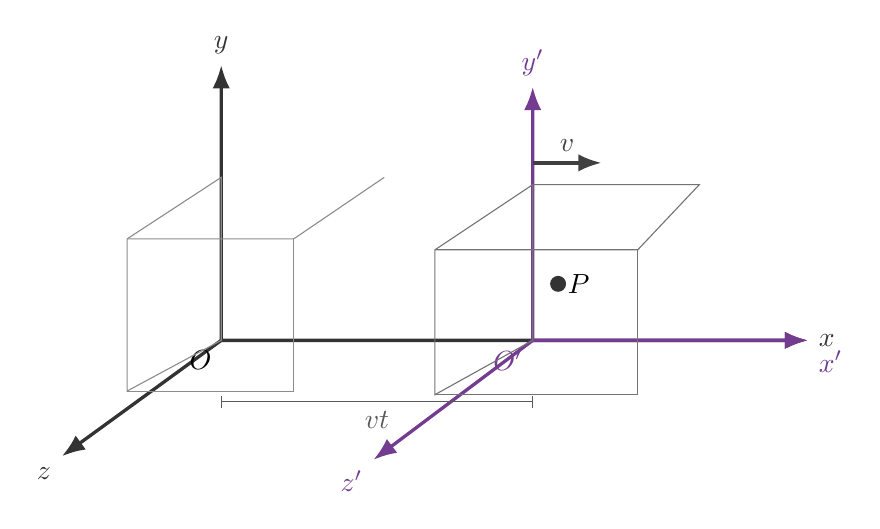
\begin{tikzpicture}[>=Latex,x=1cm,y=1cm,scale=0.92]
  % vaste assen
  \coordinate (O) at (-3.6,-0.7);
  \draw[black!80,very thick,->] (O)--(4.5,-0.7) node[right] {$x$};
  \draw[black!80,very thick,->] (O)--(-3.6,3.1) node[above] {$y$};
  \draw[black!80,very thick,->] (O)--(-5.8,-2.3) node[below left] {$z$};
  \node[below left] at (O) {$O$};

  % bewegende oorsprong en assen
  \coordinate (Op) at (0.7,-0.7);
  \draw[inkpurple,very thick,->] (Op)--(4.5,-0.7) node[below right] {$x'$};
  \draw[inkpurple,very thick,->] (Op)--(0.7,2.8) node[above] {$y'$};
  \draw[inkpurple,very thick,->] (Op)--(-1.5,-2.35) node[below left] {$z'$};
  \node[inkpurple,below left] at (Op) {$O'$};

  % afstand vt
  \draw[|-|,black!65] (-3.6,-1.55)--(0.7,-1.55)
    node[midway,below] {$vt$};

  % twee draadmodellen / blokken
  \draw[black!45] (-4.9,-1.4)--(-4.9,0.7)--(-3.6,1.55)--(-3.6,-0.7)--cycle;
  \draw[black!45] (-4.9,0.7)--(-2.6,0.7)--(-1.35,1.55);
  \draw[black!45] (-2.6,0.7)--(-2.6,-0.7);
  \draw[black!45] (-4.9,-1.4)--(-2.6,-1.4)--(-2.6,-0.7);

  \draw[black!55] (-0.65,-1.45)--(-0.65,0.55)--(0.7,1.45)--(0.7,-0.7)--cycle;
  \draw[black!55] (-0.65,0.55)--(2.15,0.55)--(3.0,1.45)--(0.7,1.45);
  \draw[black!55] (2.15,0.55)--(2.15,-0.7);
  \draw[black!55] (-0.65,-1.45)--(2.15,-1.45)--(2.15,-0.7);

  % punt en snelheid
  \fill[black!80] (1.05,0.08) circle (0.11);
  \node[right] at (1.05,0.08) {$P$};
  \draw[black!75,very thick,->] (0.7,1.75)--(1.65,1.75)
    node[midway,above] {$v$};
\end{tikzpicture}
\end{center}

\newpage
\subsection*{Rechter notitiepagina: dimensieloze Lorentzvorm}

De notitie introduceert:
\[
\beta=\frac{v}{c},
\qquad
T=c\tau.
\]

De daaropvolgende regels zijn gelezen als primed co\"ordinaten:
\begin{align*}
x' &= \gamma(x-\beta T),\\
y' &= y,\\
z' &= z,\\
T' &= \gamma(T-\beta x),\\
\gamma &= \frac{1}{\sqrt{1-\beta^2}}.
\end{align*}

\literalnote{%
De tekens bij $x'$, $y'$, $z'$ en $T'$ lijken in de scan deels op een
subscript $1$. Door de context zijn ze hier als primen weergegeven.}

% --------------------------------------------------------------------------
\newpage
\section*{PDF-pagina 22 --- fijnstructuur en onzekerheid}

\subsection*{Linker notitiepagina: fijnstructuurconstante en botsende golven}

De kop luidt ``fijnstructuur constante''. De formule staat als:
\[
\alpha=\frac{2\ell_e}{C}.
\]

Onder de formule staan twee gekleurde, elkaar naderende golfvormen. Een schuine
lijn loopt door een omcirkelde botsingszone. De labels langs deze lijn zijn
moeilijk leesbaar en lijken snelheden of richtingen aan te duiden.

\begin{center}
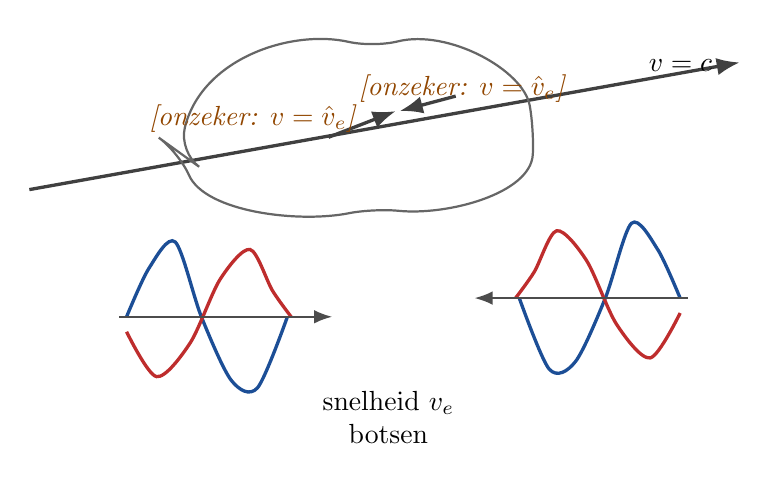
\begin{tikzpicture}[>=Latex,x=1cm,y=1cm,scale=0.95]
  % schuine baan
  \draw[black!75,very thick,->] (-4.8,1.5)--(4.7,3.2);
  \node[anchor=south west] at (3.35,2.95) {$v=c$};

  % botsingswolk
  \draw[black!60,thick,rounded corners=9pt]
    (-2.8,2.0) .. controls (-2.5,3.25) and (-1.3,3.65) ..
    (-0.2,3.4) .. controls (0.8,3.65) and (1.8,3.1) ..
    (1.95,2.3) .. controls (1.9,1.45) and (0.8,1.15) ..
    (-0.2,1.25) .. controls (-1.2,1.05) and (-2.45,1.2) ..
    cycle;
  \draw[black!75,very thick,->] (-0.8,2.2)--(0.1,2.55);
  \draw[black!75,very thick,->] (0.9,2.75)--(0.15,2.55);
  \node at (-1.8,2.45) {\uncertain{$v=\hat v_e$}};
  \node at (1.0,2.85) {\uncertain{$v=\hat v_e$}};

  % linker golfpakket
  \begin{scope}[shift={(-2.3,-0.2)}]
    \draw[inkblue,very thick]
      plot[smooth] coordinates {(-1.2,0) (-0.9,0.65) (-0.55,1.0) (-0.2,0)
                                (0.2,-0.85) (0.55,-0.95) (0.95,0)};
    \draw[inkred,very thick]
      plot[smooth] coordinates {(-1.2,-0.2) (-0.8,-0.8) (-0.35,-0.35) (0.05,0.5)
                                (0.45,0.9) (0.75,0.35) (1.0,0)};
    \draw[black!70,thick,->] (-1.3,0)--(1.55,0);
  \end{scope}

  % rechter golfpakket
  \begin{scope}[shift={(2.7,0.05)},xscale=-1]
    \draw[inkblue,very thick]
      plot[smooth] coordinates {(-1.2,0) (-0.9,0.65) (-0.55,1.0) (-0.2,0)
                                (0.2,-0.85) (0.55,-0.95) (0.95,0)};
    \draw[inkred,very thick]
      plot[smooth] coordinates {(-1.2,-0.2) (-0.8,-0.8) (-0.35,-0.35) (0.05,0.5)
                                (0.45,0.9) (0.75,0.35) (1.0,0)};
    \draw[black!70,thick,->] (-1.3,0)--(1.55,0);
  \end{scope}

  \node[align=center] at (0,-1.55) {snelheid $v_e$\\botsen};
\end{tikzpicture}
\end{center}

\literalnote{%
Links van de omcirkelde botsing staat vermoedelijk een label van de vorm
``$v=\hat v_e$''. Ook het korte label aan het begin van de schuine lijn is
niet eenduidig leesbaar.}

\newpage
\subsection*{Rechter notitiepagina: onzekerheidsprincipe van Heisenberg}

De kop luidt ``Onzekerheids principe Heisenberg''. De eerste zin is:
\literalnote{%
Je weet nooit de exacte locatie en snelheid van een elektron.}

Daarna volgt, zo letterlijk mogelijk:
\literalnote{%
Daar waar de golf \uncertain{inklapt}, \uncertain{heb je dat het met de
snelheid gaat}. Hoe hoger de frequentie, hoe exacter de locatie.}

Onder de tekst staat een gearceerde bol met het label ``bubbel'' en daaronder
``$K_2$''.

\begin{center}
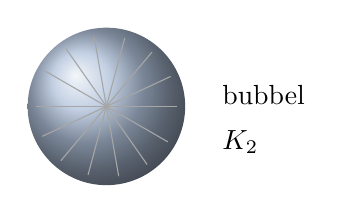
\begin{tikzpicture}[x=1cm,y=1cm]
  \shade[ball color=inkblue!35] (0,0) circle (1.0);
  \foreach \a in {0,25,...,155}
    \draw[black!35] ({-0.9*cos(\a)},{-0.9*sin(\a)})
      -- ({0.9*cos(\a)},{0.9*sin(\a)});
  \node[right=1.35cm] at (0,0.15) {bubbel};
  \node[right=1.35cm] at (0,-0.45) {$K_2$};
\end{tikzpicture}
\end{center}

% --------------------------------------------------------------------------
\newpage
\section*{PDF-pagina 23 --- stroom, spanning en rechterhandregel}

\subsection*{Linker notitiepagina: stroom door een draad}

De titel luidt ``Stroom door een draad''. Een elektron beweegt in de tekening
van een negatief naar een positief geladen uiteinde.

\begin{center}
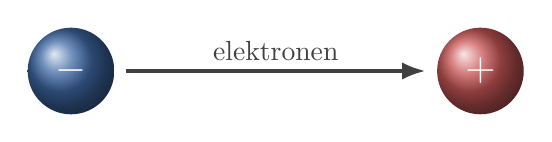
\begin{tikzpicture}[>=Latex,x=1cm,y=1cm]
  \shade[ball color=inkblue!85] (-2.6,0) circle (0.55);
  \node[white,font=\bfseries\Large] at (-2.6,0) {$-$};
  \shade[ball color=inkred!80] (2.6,0) circle (0.55);
  \node[white,font=\bfseries\Large] at (2.6,0) {$+$};
  \draw[black!75,very thick,->] (-1.9,0)--(1.9,0)
    node[midway,above] {elektronen};
\end{tikzpicture}
\end{center}

De elementaire lading staat als:
\[
1\ \text{elektron}=e\approx1{,}6\times10^{-19}\ \mathrm{Coulomb}.
\]

Voor de stroomsterkte wordt genoteerd:
\[
I=\frac{\Delta Q}{\Delta t}
 =\frac{C}{T}
 =\mathrm{ampere},
\qquad
\frac{N_{\text{elektronen}}}{\mathrm{sec}}.
\]

Voor de spanning staat:
\[
V=\frac{W}{Q}
 =\frac{\mathrm{joule}}{\mathrm{coulomb}}
 =\mathrm{volt}.
\]

\newpage
\subsection*{Rechter notitiepagina: rechterhandregel en elektronenverzameling}

Bovenaan staat ``Rechter hand regel''. De bovenste schets toont een rode
stroomas van min naar plus en blauwe cirkelvormige veldlijnen.

\begin{center}
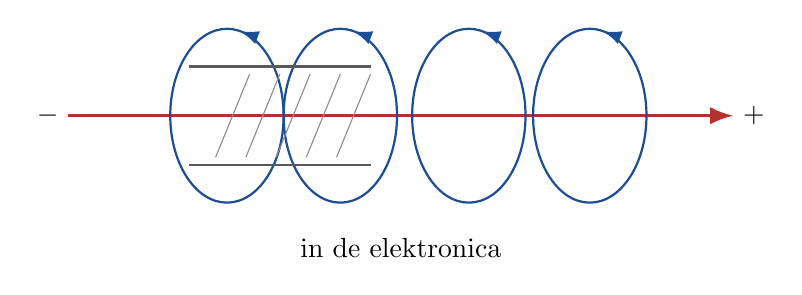
\begin{tikzpicture}[>=Latex,x=1cm,y=1cm,scale=0.96]
  \draw[inkred,very thick,->] (-4.4,0)--(4.4,0);
  \node[left] at (-4.4,0) {$-$};
  \node[right] at (4.4,0) {$+$};

  \foreach \x in {-2.3,-0.8,0.9,2.5} {
    \draw[inkblue,thick,
      postaction={decorate},
      decoration={markings,mark=at position .22 with {\arrow{Latex}}}]
      (\x,0) ellipse (0.75 and 1.15);
  }
  \draw[black!65,thick] (-2.8,0.65)--(-0.4,0.65);
  \draw[black!65,thick] (-2.8,-0.65)--(-0.4,-0.65);
  \foreach \x in {-2.45,-2.05,-1.65,-1.25,-0.85}
    \draw[black!45] (\x,-0.55)--({\x+0.45},0.55);

  \node at (0,-1.75) {in de elektronica};
\end{tikzpicture}
\end{center}

De tweede schets toont een langwerpige geleider met min links en plus rechts.
Blauwe pijlen en een compacte wolk bij de minzijde stellen verzamelde
elektronen voor.

\begin{center}
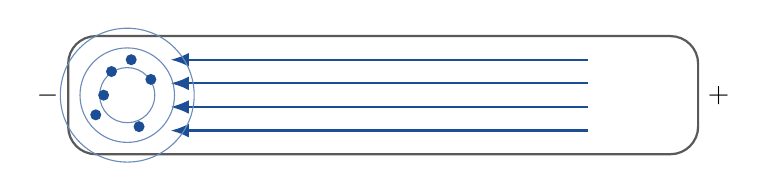
\begin{tikzpicture}[>=Latex,x=1cm,y=1cm]
  \draw[black!65,thick,rounded corners=10pt]
    (-4,-0.75) rectangle (4,0.75);
  \node[left] at (-4,0) {$-$};
  \node[right] at (4,0) {$+$};

  \foreach \y in {-0.45,-0.15,0.15,0.45}
    \draw[inkblue,thick,->] (2.6,\y)--(-2.7,\y);
  \foreach \r in {0.35,0.6,0.85}
    \draw[inkblue!65] (-3.25,0) circle (\r);
  \foreach \p in {(-3.65,-0.25),(-3.45,0.3),(-3.1,-0.4),(-2.95,0.2),
                  (-3.55,0.0),(-3.2,0.45)}
    \fill[inkblue] \p circle (0.07);
\end{tikzpicture}
\end{center}

De tekst eronder luidt:
\literalnote{%
In de kwantum natuurkunde gaan de elektronen zich verzamelen op de
min-onderdelen.}

% --------------------------------------------------------------------------
\newpage
\section*{PDF-pagina 24 --- supergeleiding en lokalisatie}

\subsection*{Linker notitiepagina: geleider, supergeleider en Meissnereffect}

De bladzijde vergelijkt twee situaties. Bovenaan staat ``Supergeleiding''.
Een bolvormig voorwerp beweegt naar een magneet met noordpool $N$; groene
veldlijnen lopen door en om het systeem. Deze bovenste situatie is gelabeld
``geleidende metaal'', ``Situatie'' en ``Flux lijn''.

\begin{center}
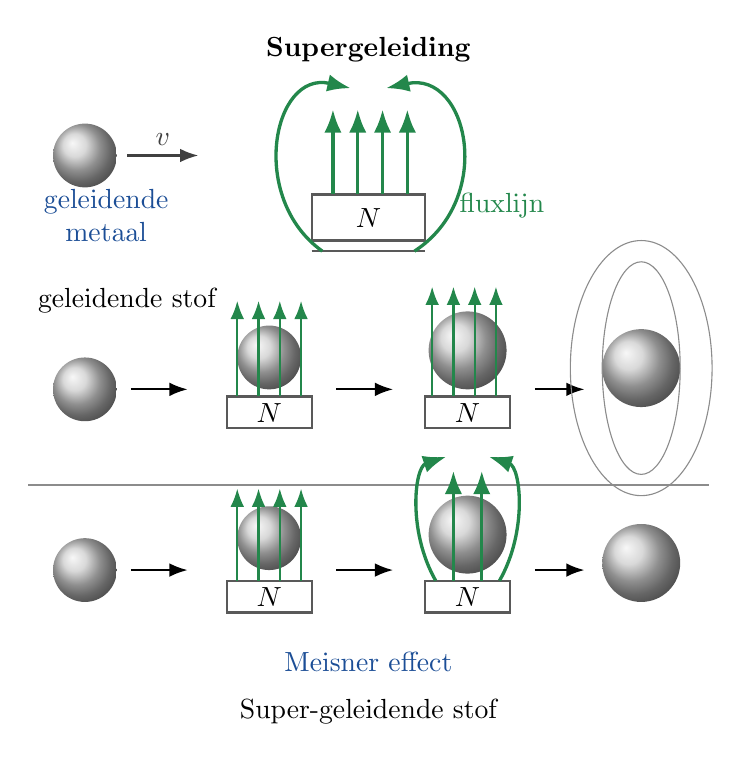
\begin{tikzpicture}[>=Latex,x=1cm,y=1cm,scale=0.90]
  % eerste situatie
  \node[font=\bfseries] at (0,4.1) {Supergeleiding};
  \shade[ball color=black!20] (-4.0,2.6) circle (0.45);
  \draw[black!75,thick,->] (-3.4,2.6)--(-2.4,2.6) node[midway,above] {$v$};
  \node[inkblue,align=center] at (-3.7,1.75) {geleidende\\metaal};

  \draw[black!65,thick] (-0.8,1.4) rectangle (0.8,2.05);
  \node at (0,1.72) {$N$};
  \draw[black!65,thick] (-0.8,1.25)--(0.8,1.25);

  \foreach \x in {-0.5,-0.15,0.2,0.55}
    \draw[inkgreen,very thick,->] (\x,2.05)--(\x,3.25);
  \draw[inkgreen,very thick,->]
    (-0.65,1.25) .. controls (-1.7,2.0) and (-1.35,3.8) .. (-0.25,3.55);
  \draw[inkgreen,very thick,->]
    (0.65,1.25) .. controls (1.8,2.0) and (1.4,3.8) .. (0.25,3.55);
  \node[inkgreen,anchor=west] at (1.15,1.9) {fluxlijn};

  % overgangsreeks geleidend
  \node[anchor=west] at (-4.8,0.55) {geleidende stof};
  \shade[ball color=black!20] (-4.0,-0.7) circle (0.45);
  \draw[->,thick] (-3.35,-0.7)--(-2.55,-0.7);
  \draw[black!65,thick] (-2.0,-1.25) rectangle (-0.8,-0.8);
  \node at (-1.4,-1.03) {$N$};
  \shade[ball color=black!20] (-1.4,-0.25) circle (0.45);
  \foreach \x in {-1.85,-1.55,-1.25,-0.95}
    \draw[inkgreen,thick,->] (\x,-0.8)--(\x,0.55);

  \draw[->,thick] (-0.45,-0.7)--(0.35,-0.7);
  \draw[black!65,thick] (0.8,-1.25) rectangle (2.0,-0.8);
  \node at (1.4,-1.03) {$N$};
  \shade[ball color=black!20] (1.4,-0.15) circle (0.55);
  \foreach \x in {0.9,1.2,1.5,1.8}
    \draw[inkgreen,thick,->] (\x,-0.8)--(\x,0.75);

  \draw[->,thick] (2.35,-0.7)--(3.05,-0.7);
  \shade[ball color=black!20] (3.85,-0.4) circle (0.55);
  \draw[black!45] (3.85,-0.4) ellipse (1.0 and 1.8);
  \draw[black!45] (3.85,-0.4) ellipse (0.55 and 1.5);

  % scheiding
  \draw[black!45] (-4.8,-2.05)--(4.8,-2.05);

  % Meissnerreeks
  \shade[ball color=black!20] (-4.0,-3.25) circle (0.45);
  \draw[->,thick] (-3.35,-3.25)--(-2.55,-3.25);
  \draw[black!65,thick] (-2.0,-3.85) rectangle (-0.8,-3.4);
  \node at (-1.4,-3.63) {$N$};
  \shade[ball color=black!20] (-1.4,-2.8) circle (0.45);
  \foreach \x in {-1.85,-1.55,-1.25,-0.95}
    \draw[inkgreen,thick,->] (\x,-3.4)--(\x,-2.1);

  \draw[->,thick] (-0.45,-3.25)--(0.35,-3.25);
  \draw[black!65,thick] (0.8,-3.85) rectangle (2.0,-3.4);
  \node at (1.4,-3.63) {$N$};
  \shade[ball color=black!20] (1.4,-2.75) circle (0.55);
  \draw[inkgreen,very thick,->]
    (0.95,-3.4) .. controls (0.55,-2.7) and (0.65,-1.8) .. (1.1,-1.65);
  \draw[inkgreen,very thick,->]
    (1.85,-3.4) .. controls (2.25,-2.7) and (2.15,-1.8) .. (1.7,-1.65);
  \draw[inkgreen,very thick,->] (1.2,-3.4)--(1.2,-1.85);
  \draw[inkgreen,very thick,->] (1.6,-3.4)--(1.6,-1.85);

  \draw[->,thick] (2.35,-3.25)--(3.05,-3.25);
  \shade[ball color=black!20] (3.85,-3.15) circle (0.55);

  \node[inkblue] at (0,-4.55) {Meisner effect};
  \node at (0,-5.25) {Super-geleidende stof};
\end{tikzpicture}
\end{center}

\literalnote{%
De scan schrijft ``Meisner effect''. De gangbare spelling is
\textit{Meissnereffect}.}

\newpage
\subsection*{Rechter notitiepagina: waarom de supergeleider wordt gelockt}

De vraag bovenaan luidt:
\literalnote{%
Waarom word de supergeleider gelocked op de locatie?}

De tekening toont rode atoomkernen in een gezamenlijke blauwe elektronenwolk.

\begin{center}
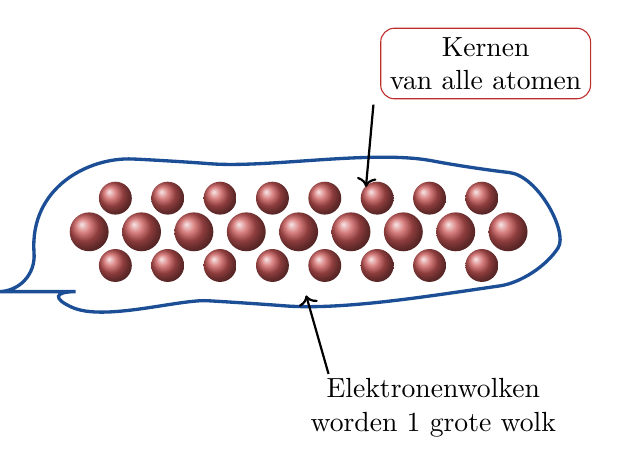
\begin{tikzpicture}[x=1cm,y=1cm,scale=0.95]
  \draw[inkblue,very thick,rounded corners=14pt]
    (-3.5,-0.8) .. controls (-2.6,-1.2) and (-1.6,-0.9) ..
    (-0.7,-0.95) .. controls (0.6,-1.05) and (1.8,-0.85) ..
    (3.2,-0.65) .. controls (3.6,0.0) and (3.2,0.75) ..
    (2.3,0.85) .. controls (1.0,1.1) and (-0.4,0.85) ..
    (-1.7,0.95) .. controls (-2.8,1.0) and (-3.6,0.6) ..
    cycle;
  \foreach \x in {-2.8,-2.1,-1.4,-0.7,0,0.7,1.4,2.1,2.8}
    \shade[ball color=inkred!80] (\x,0) circle (0.26);
  \foreach \x in {-2.45,-1.75,-1.05,-0.35,0.35,1.05,1.75,2.45}
    \shade[ball color=inkred!80] (\x,0.45) circle (0.22);
  \foreach \x in {-2.45,-1.75,-1.05,-0.35,0.35,1.05,1.75,2.45}
    \shade[ball color=inkred!80] (\x,-0.45) circle (0.22);

  \draw[->,thick] (1.0,1.7)--(0.9,0.6);
  \node[draw=inkred,rounded corners=5pt,align=center] at (2.5,2.25)
    {Kernen\\van alle atomen};

  \draw[->,thick] (0.4,-1.9)--(0.1,-0.85);
  \node[align=center] at (1.8,-2.35)
    {Elektronenwolken\\worden 1 grote wolk};
\end{tikzpicture}
\end{center}

De toelichting luidt:
\literalnote{%
Tijdens de kwantum excitatie klapt de hele wolk in op 1 positie, i.p.v.
meerdere op verschillende plekken.}

% --------------------------------------------------------------------------
\newpage
\section*{PDF-pagina 25 --- Coulombkracht en harmonische beweging}

\subsection*{Linker notitiepagina: verzameling formules en numerieke waarden}

De eerste vergelijking is aangeduid als ``formule Coulomb'':
\[
F=\frac{Q^2}{4\pi\varepsilon_0}\left(\frac{1}{x}\right).
\]

\noindent
In de gebruikelijke Coulombwet staat $1/x^2$; de scan toont hier duidelijk
$1/x$, en dat is daarom letterlijk behouden.

De overige relaties staan als:
\begin{align*}
E &= \frac{1}{2}Kx^2, &
K &= \frac{F_{\max}}{x_{\max}},\\
f &= \frac{\omega}{2\pi}, &
\omega &= \sqrt{\frac{k}{m}},\\
V &= f\,x, &
\omega &= \frac{V}{R}.
\end{align*}

De genoteerde waarden zijn:
\begin{align*}
R_{\text{kern}} &= 1{,}36\times10^{-15}\ \mathrm{m},\\
F_{\max} &= 29{,}053507333\ \mathrm{N}.
\end{align*}

Een brede, doorgestreepte numerieke uitwerking in het midden is niet
betrouwbaar leesbaar en is daarom niet gereconstrueerd. Onderaan staat:
\[
V_e=
\left(\frac{R_c}{\pi}\right)
\sqrt{\frac{F_{\max}}{2R_km_k}}.
\]

\newpage
\subsection*{Rechter notitiepagina: snelheid uit veerconstante}

Bovenaan staat een afzonderlijke relatie. De plaats van $R_c$ buiten de
wortel is in de scan enigszins onduidelijk; de meest waarschijnlijke lezing is:
\[
V_e=
\sqrt{\frac{k_{\text{spring constant}}}{m_{\text{electron}}}}\;R_c.
\]

Daaronder staat een omkaderde samenvatting:
\begin{center}
\fbox{%
\begin{minipage}{0.52\linewidth}
\begin{align*}
V &= f\,x,\\
f &= \frac{1}{2\pi}\omega,\\
\omega &= \sqrt{\frac{k}{m}},\\
K &= \frac{F_{\max}}{x_{\max}}.
\end{align*}
\end{minipage}}
\end{center}

\literalnote{%
In deze bladzijde worden zowel $K$ als $k$ gebruikt voor een veerconstante.
Hoofdletters, kleine letters en subscripten zijn behouden zoals ze in de scan
staan.}

\end{document}
